\documentclass[aspectratio=169]{beamer}

\usepackage[english]{babel}
\usepackage[utf8x]{inputenc}			
\usepackage{listings}
\usepackage{xcolor}

\lstdefinestyle{Rstyle}{
  language=R,
  basicstyle=\ttfamily\footnotesize,
  keywordstyle=\color{blue!70!black}\bfseries,
  commentstyle=\color{gray!70!black}\itshape,
  stringstyle=\color{orange!80!black},
  numbers=left,
  numberstyle=\tiny\color{gray},
  numbersep=6pt,
  showstringspaces=false,
  breaklines=true,
  frame=single,
  rulecolor=\color{gray!40},
  backgroundcolor=\color{gray!5},
  tabsize=2,
  morekeywords={aov, summary, factor, data.frame, head, str}
}
\lstset{style=Rstyle}
\usepackage{xcolor}
\usepackage{tikz}
\usetikzlibrary{shapes.geometric, arrows.meta, positioning}

\usetikzlibrary{trees}  % 用於樹狀圖
\lstset{
    language=R,
    basicstyle=\ttfamily\small,
    backgroundcolor=\color{gray!10},
    frame=single,
    breaklines=true,
    showstringspaces=false,
    keywordstyle=\color{blue},
    commentstyle=\color{green!50!black},
    stringstyle=\color{red},
    numbers=none,
    xleftmargin=10pt,
    xrightmargin=10pt,
    framexleftmargin=5pt,
    framexrightmargin=5pt
}

\mode<presentation>						
{
  \usetheme{default}					
  \usecolortheme{default} 			
  \usefonttheme{default}  				
  \setbeamertemplate{caption}[numbered]	
}

\usepackage{graphicx}
\graphicspath{{figure/}}				% Shared figure folder for all labs
\usepackage{booktabs}
\usepackage{hyperref}					
\usepackage{subcaption}  
\usepackage{multicol}
\usepackage{hyperref}

\title{Regression Analysis}	
\author{Rex Shao-Yu Wang}								
\institute{Department of Agronomy, National Taiwan University}				
\date{May 25, 2026}								

\begin{document}

% Title page
\begin{frame}
  \titlepage
\end{frame}

% Outline
\begin{frame}{Outline}
  \tableofcontents
\end{frame}


\section{Correlation}

% ====================== Frame 1 ======================
\begin{frame}[fragile]{Covariance}
The \textbf{Covariance} between two variables can be estimated by:

\begin{align*}
    cov(X,Y) &= s_{xy} = \frac{1}{n-1}\sum_{i=1}^n (x_i - \overline{x})(y_i - \overline{y}) 
\end{align*} 

\begin{block}{Code}
\begin{lstlisting}
cov(fert$Fertiliser, fert$Yield)
cov(fert$Yield, fert$Fertiliser)
\end{lstlisting}
\end{block}

\begin{exampleblock}{Output}
\begin{lstlisting}[numbers=none]
> cov(fert$Fertiliser, fert$Yield)
[1] 25.54167
> cov(fert$Yield, fert$Fertiliser)
[1] 25.54167
\end{lstlisting}
\end{exampleblock}

\end{frame}


% ====================== Frame 2 ======================
\begin{frame}[fragile]{Correlation Coefficient}
\textbf{Pearson’s correlation} measure standardizes the covariance by the variances of the original variables, so that its value always falls between \textbf{-1 and +1}.
It is defined as:
{\large
\begin{align*}
	r_{XY} = \frac{S_{XY}}{\sqrt{S^2_X S^2_Y}} = \frac{S_{XY}}{S_XS_Y}
\end{align*}}

\begin{block}{Code}
\begin{lstlisting}
cor(fert$Fertiliser, fert$Yield)
\end{lstlisting}
\end{block}

\begin{exampleblock}{Output}
\begin{lstlisting}[numbers=none]
> cor(fert$Fertiliser, fert$Yield)
[1] 0.8559683
\end{lstlisting}
\end{exampleblock}
\end{frame}



% ====================== Frame 3 ======================
\begin{frame}{Test of significance for correlation}
A method that tests whether a sample correlation coefficient ($r$) could have come from a population with \textbf{zero correlation} ($\rho = 0$), i.e., whether the two variables are truly associated. \\
\vspace{5pt}
\textbf{Hypothesis:}
\[
\begin{aligned}
H_0 &: \rho = 0 \quad \text{(the two variables are uncorrelated)}\\
H_1 &: \rho \neq 0
\end{aligned}
\]
\vspace{2pt}
\textbf{Test Statistic:}
\[
t_0 = \frac{r - 0}{SE(r)} = r \sqrt{\frac{n-2}{1 - r^2}}
\]
where $SE(r) = \sqrt{\dfrac{1 - r^2}{n - 2}}$ is the standard error of $r$, with $df = n - 2$.\\
\vspace{6pt}
\textbf{Decision Rule:}\\
Reject $H_0$ if \ $|t_0| > t_{\alpha/2,\, n-2}$ \quad (the correlation is significant).\\
\end{frame}


% ====================== Frame 4 ======================
\begin{frame}[fragile]{Test of significance for correlation}
\begin{block}{Code}
\begin{lstlisting}
cor.test(fert$Fertiliser, fert$Yield)
\end{lstlisting}
\end{block}
\begin{exampleblock}{Output}
\begin{figure}
    \centering
    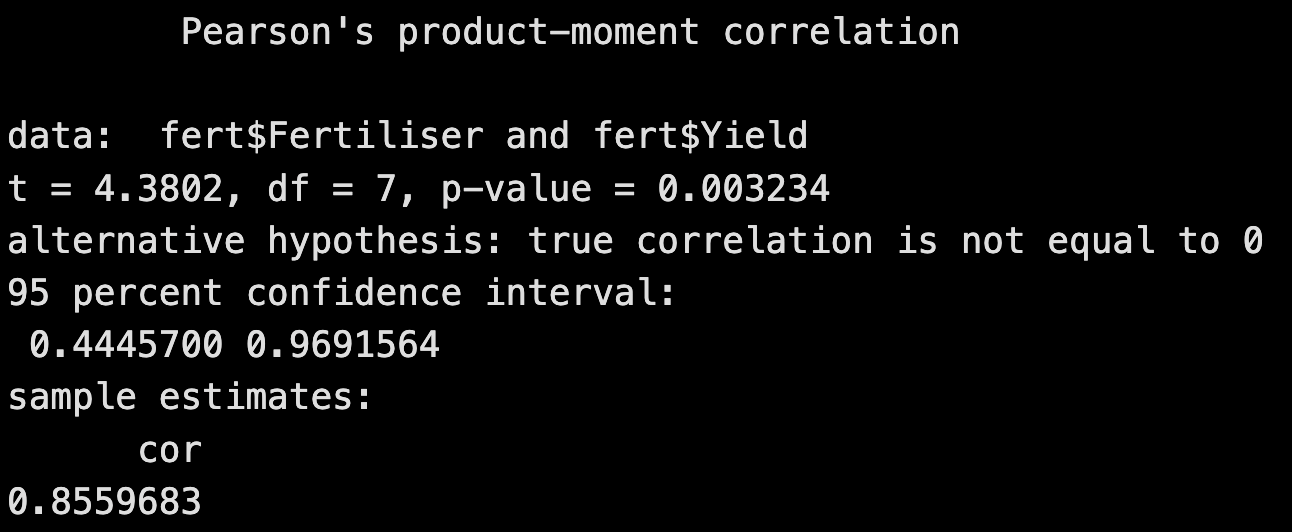
\includegraphics[width=0.8\linewidth]{Screenshot 2026-05-23 at 12.42.44 AM.png}
\end{figure}
\end{exampleblock}
\end{frame}



% ====================== Regression ======================
\section{Regression}

% ---------- 第 1 頁：線性方程式 + lm 輸出 ----------
\begin{frame}[fragile]{Fitting a linear model in R}
The simple linear regression model:
\[
\hat{y}_i = a + b\,x_i
\]
where $a$ is the intercept and $b$ is the slope. We use \texttt{lm()} to estimate $a$ and $b$.\\
\vspace{4pt}
\begin{block}{Code}
\begin{lstlisting}
model <- lm(Mortality ~ Exposure, data = mort)
model
\end{lstlisting}
\end{block}
\begin{exampleblock}{Output}
\begin{lstlisting}[numbers=none]
Call:
lm(formula = Mortality ~ Exposure, data = mort)

Coefficients:
(Intercept)     Exposure  
    114.716        9.231  
\end{lstlisting}
\end{exampleblock}
\[
\Rightarrow \quad \hat{y}_i = 114.716 + 9.231\,x_i
\]
\end{frame}


% ---------- 第 2 頁：拆解 summary 上半 (係數表) ----------
\begin{frame}[fragile]{Reading the output: coefficients}
\begin{block}{Code}
\begin{lstlisting}
summary(model)
\end{lstlisting}
\end{block}
\begin{exampleblock}{Output (coefficients)}
\begin{lstlisting}[numbers=none]
            Estimate Std. Error t value Pr(>|t|)    
(Intercept)  114.716      8.046  14.258 1.98e-06 ***
Exposure       9.231      1.419   6.507 0.000332 ***
\end{lstlisting}
\end{exampleblock}
\begin{block}{What each number means (for \texttt{Exposure})}
\begin{itemize}
  \item \texttt{Estimate} $= 9.231$ \quad $\rightarrow$ \ slope $b$
  \item \texttt{Std. Error} $= 1.419$ \quad $\rightarrow$ \ $SE(b)$
  \item \texttt{t value} $= 6.507$ \quad $\rightarrow$ \ $t_0 = b / SE(b)$
  \item \texttt{Pr(>|t|)} $= 0.0003$ \quad $\rightarrow$ \ $p$-value for $H_0: \beta = 0$
\end{itemize}
\end{block}
\end{frame}


% ---------- 第 3 頁：r^2 公式與定義 ----------
\begin{frame}{Coefficient of determination ($r^2$)}
How much of the variability in $Y$ is explained by $X$?
\[
r^2 = \frac{SS_{Reg ression}}{SS_{Total}}
\]
\textbf{Definition:} the proportion of the total variability in $Y$ that is explained by the regression on $X$.\\
\vspace{6pt}
\begin{itemize}
  \item $r^2 \to 1$: the model explains most of the variability.
  \item $r^2 \to 0$: the model explains very little.
  \item Note: \ $\sqrt{r^2} = |r|$ \ (links regression back to correlation).
\end{itemize}
\end{frame}

\begin{frame}{Adjusted $r^2$}
Why not just use $r^2$? Adding more predictors \textbf{always} increases $r^2$, even useless ones.
\[
r^2_{adj} = 1 - (1 - r^2)\,\frac{n - 1}{n - k - 1}
\]
\textbf{Definition:} a version of $r^2$ that is penalised for the number of predictors ($k$) in the model.\\
\vspace{6pt}
\begin{itemize}
  \item It only increases if a new predictor improves the model more than expected by chance.
  \item $r^2_{adj} \leq r^2$ \ (always equal to or smaller than $r^2$).
  \item Useful for comparing models with different numbers of predictors.
\end{itemize}
\end{frame}


% ---------- 第 4 頁：F 檢定在做什麼 ----------
\begin{frame}{The F-test in regression}
The total variation in $Y$ is partitioned into two parts:
\[
SS_{Total} = SS_{Regression} + SS_{Residual}
\]
The \textbf{F-test} compares the \emph{explained} variation against the \emph{unexplained} variation:
\[
F_0 = \frac{MS_{Regression}}{MS_{Residual}}
\]
\textbf{Hypothesis:}
\[
H_0 : \beta = 0 \qquad H_1 : \beta \neq 0
\]
A large $F_0$ (small $p$-value) means $X$ explains significantly more variation than random error $\Rightarrow$ reject $H_0$.

\vspace{4pt}
\textbf{Note:} For simple linear regression (one $X$), the F-test and the
slope $t$-test are equivalent: \ $F_0 = t_0^2 = 6.507^2 = 42.34$, \ same $p$-value.
\end{frame}


% ---------- 第 5 頁：拆解 summary 下半 (模型整體) ----------
\begin{frame}[fragile]{Reading the output: model fit}
\begin{exampleblock}{Output (bottom of summary)}
\begin{lstlisting}[numbers=none]
Multiple R-squared:  0.8581,  Adjusted R-squared:  0.8378 
F-statistic: 42.34 on 1 and 7 DF,  p-value: 0.0003321
\end{lstlisting}
\end{exampleblock}
\begin{block}{What each number means}
\begin{itemize}
  \item \texttt{R-squared} $= 0.858$ \ $\rightarrow$ \ $X$ explains 85.8\% of the variability in $Y$
  \item $\sqrt{0.858} \approx 0.926$ \ $\rightarrow$ \ the correlation coefficient $r$
  \item \texttt{F-statistic} $= 42.34$, \ $p = 0.0003$ \ $\rightarrow$ \ result of the F-test ($H_0: \beta = 0$)
\end{itemize}
\end{block}
\begin{alertblock}{Conclusion}
$F_0 = 42.34$, $p < 0.05$ $\Rightarrow$ Reject $H_0$.\\
Exposure explains a significant proportion of the variability in mortality.
\end{alertblock}
\end{frame}


% ---------- 第 6 頁：把配適線畫在圖上 ----------
\begin{frame}[fragile]{Plotting the fitted line}
Once we have the model, we can draw the fitted line on the scatter plot using \texttt{abline()}.\\
\vspace{4pt}
\begin{block}{Code}
\begin{lstlisting}
plot(mort$Exposure, mort$Mortality,
     xlab = "Exposure", ylab = "Mortality")
abline(model, col = "red")
\end{lstlisting}
\end{block}
\vspace{2pt}
\begin{itemize}
  \item \texttt{plot()} draws the data points.
  \item \texttt{abline(model)} adds the regression line directly from the fitted model.
\end{itemize}
\end{frame}




\section{Lab Report}
\begin{frame}{Lab Report}
\begin{itemize}
    \item The report file will be in the NTU COOL Assignment section
    \item Submit your file in pdf format
    \item Deadline: 5/31 (Sun) 23:59
    \item Late submission is not accepted
\end{itemize}
\end{frame}
\end{document}




